\section{Ejercicio 7}
Los circuitos capaces de realizar operaciones aritméticas son pilares esenciales para la contrucción de distintos circuitos lógicos de aplicación. Mediante el uso de distintas compuertas es posible diseñar circuitos capaces de realizar la operación arimética más básica: la suma. Los contadores lógicos, son circuitos capaces de incrementar o decrementar de a una unidad. Existen basicamente dos tipos de contadores: los sincrónicos y los asincrónicos. La diferencia esencial entre ambos es que en los sincrónicos todos los elementos de memoria responden a un solo clock en simultáneo, mientras que los asincrónicos funcionan en cascada, lo que genera retrasos medibles en el cambio de estado del contador. 


Debido a que los flip-flops que forman parte de los contadores se logran mediante la implementación correcta de transistores, los cambios de estado no son instantáneos. Se pueden definir distintos tiempos físicos que reflejan el comportamiento real de un flip-flop y de un contador o un circuito lógico en general. El tiempo de propagación o propagation delay time en inglés, es el tiempo que le toma a la salida del circuito reflejar un cambio en la entrada, por ejemplo, un flanco positivo del clock. Este par\'ametro dictar\'a entonces la m\'axima velocidad de operaci\'on de un contador. 

\subsection{Contador asincrónico} 

Una manera de implementar un contador que cuente hacia arriba es mediante el uso de flip flops tipo T. El siguiente circuito es un contador asincrónico de 3 bits, capaz de contar hasta 7:

\begin{figure}[H]
	\centering
	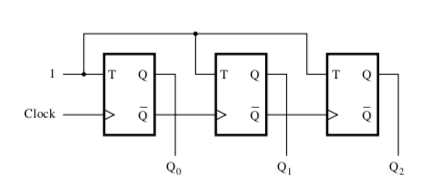
\includegraphics[width=0.8\textwidth]{Ejercicio7/Recursos/asincronico}
	\caption{Contador asincrónico}
\end{figure}

En el circuito se conectan los tres flip-flops en cascada, de ahí que sea asincrónico. La entradas de cada uno esta conectada a una señal constante igual a $1$, y por ende la salida de cada uno se invierte con cada flanco ascendente del Clock. Los últimos dos flip-flops están conectados a la salida $\bar{Q}$ correspondiente, por lo que cambian su estado siempre que la salida del anterior pase de $Q = 1$ a $Q = 0$, es decir un flanco positivo en $\bar{Q}$. Una desventaja clara de este tipo de circuitos es el delay de propagación. Debido a que los flip-flops están configurados en cadena, para observar un cambio a la salida del último de ellos, la señal debe pasar por todos los anteriores, por ende habrá un retraso medible que hace poco práctica la implementación de este tipo de circuitos cuando se quiere contar grandes cifras. 


Se espera para este circuito que el tiempo de propagaci\'on total sea la suma de la propagaci\'on individual de cada flip-flop, para el integrado realizado $ns$.


\subsection{Contador sincrónico}

Un contador sincr\'onico posible es el siguiente:


\begin{figure}[H]
	\centering
	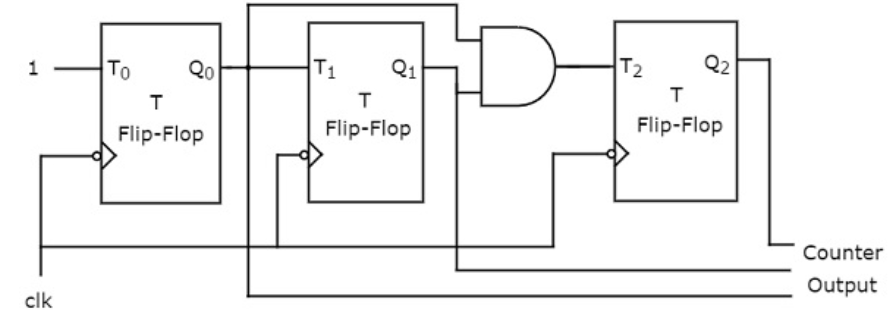
\includegraphics[width=0.8\textwidth]{Ejercicio7/Recursos/sincronico}
	\caption{Contador asincrónico}
\end{figure}

el ciruito contiene 3 flip-flops T, una compuerta And de dos entradas y es activado por un flanco descendente del clock. Siempre que incida un  flanco descendente se prende la salida del prier flip-flop, mientras que la salida del segundo es igual a 1 siempre que $Q_0$ sea igual a 1 e incida el flanc corespondiente. Luego $Q_2$ ser\'a igual a 1 cuando se reciba un clock corrspondiente y tanto $Q_0$ como $Q_1$ sean positivas y as\'i se logra contar hacia arriba. Para este circuito, se esperan tiempos de propagaci\'on menores que en el contador asincr\'onico y por ende una velocidad de operaci\'on mayor. 

\subsection{Mediciones}

Para el contador asincrónico se midió la propagación desde el clock a cada flip-flop y por último la propagación total(hasta $Q_3$):

\begin{table}[H]
\centering
\begin{tabular}{lll}\hline
Propagación $CLK$-$Q_1$($ns$) & Propagacion $Q_1$-$Q_2$($ns$) & Propagación $Q_2$-$Q_3$($ns$)\\ \hline
$90$  &       $177$ & $250$  \\ \hline

\end{tabular}
\end{table}

En la siguiente figura puede verse el tiempo de propagación entre el clock y el primer flip-flop

\begin{figure}[H]
	\centering
	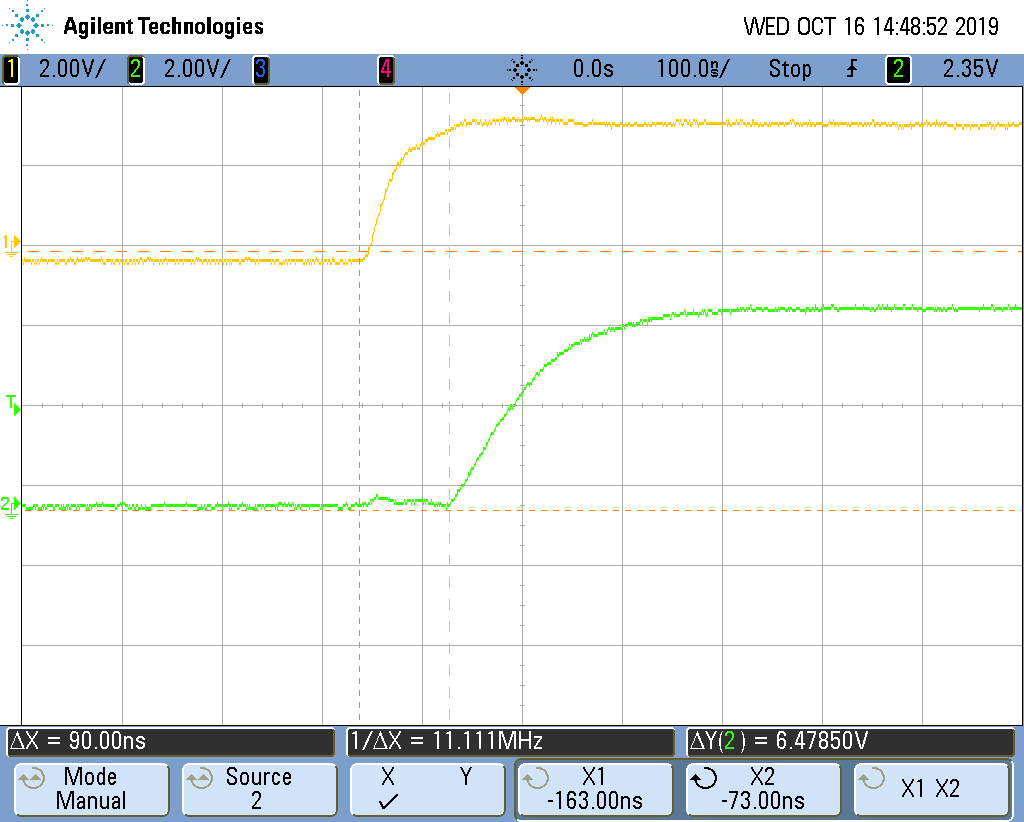
\includegraphics[width=0.8\textwidth]{Ejercicio7/Recursos/propagacion_asincronico.png}
	\caption{Propagacion asincronico}
\end{figure}

A continuación se adjunta una captura de osciloscopio que contiene tanto la señal de clock (canal 1) y las salidas del primero, segundo y tercer flip-flop (canal 2, 4, y 3 respectivamente). 

\begin{figure}[H]
	\centering
	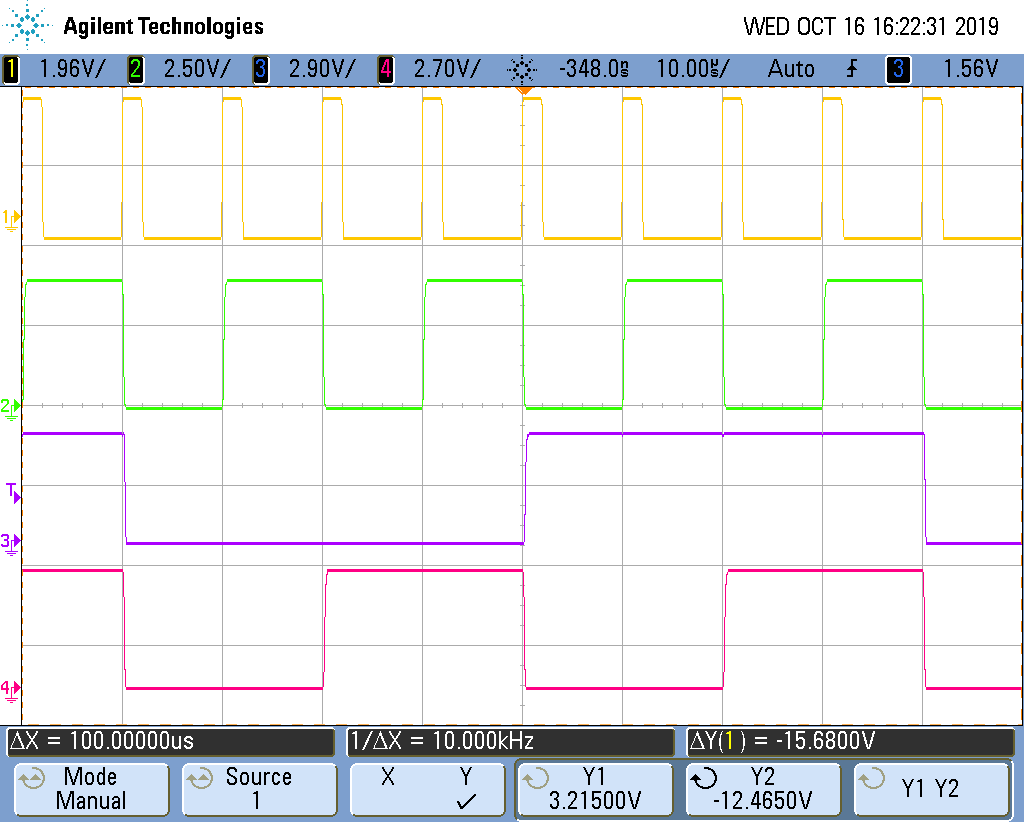
\includegraphics[width=0.8\textwidth]{Ejercicio7/Recursos/senales_asincronico.png}
	\caption{Propagacion asincronico}
\end{figure}

Puede verse como cada salida ocurre con el retraso de clock correpondiente a cada flip-flop, representando un 1 binario en el orden adecuado del contador. Este diagrama de tiempo es una muy buena manera de ver cuando se prende cada flip-flip y comprender como se realiza el proceso de conteo. Cuando un flanco acendente de reloj incide se prende el primer flip-flop, luego al siguiente lo hace el segundo, y dos después el tercero, confirmando el funcionamiento antes explicado. En este caso se sacrifica velocidad de funcionamiento ya que se debe esperar a cada flanco de clock y que el mismo se propague para realizar el conteo. Por ende la máxima velocidad de operación está dada por ese tiempo de propagación, para el circuito realizado $250ns$.

Por otro lado, en el caso del contador sncr\'onico se midi\'o la propgaci\'on total:


\begin{figure}[H]
	\centering
	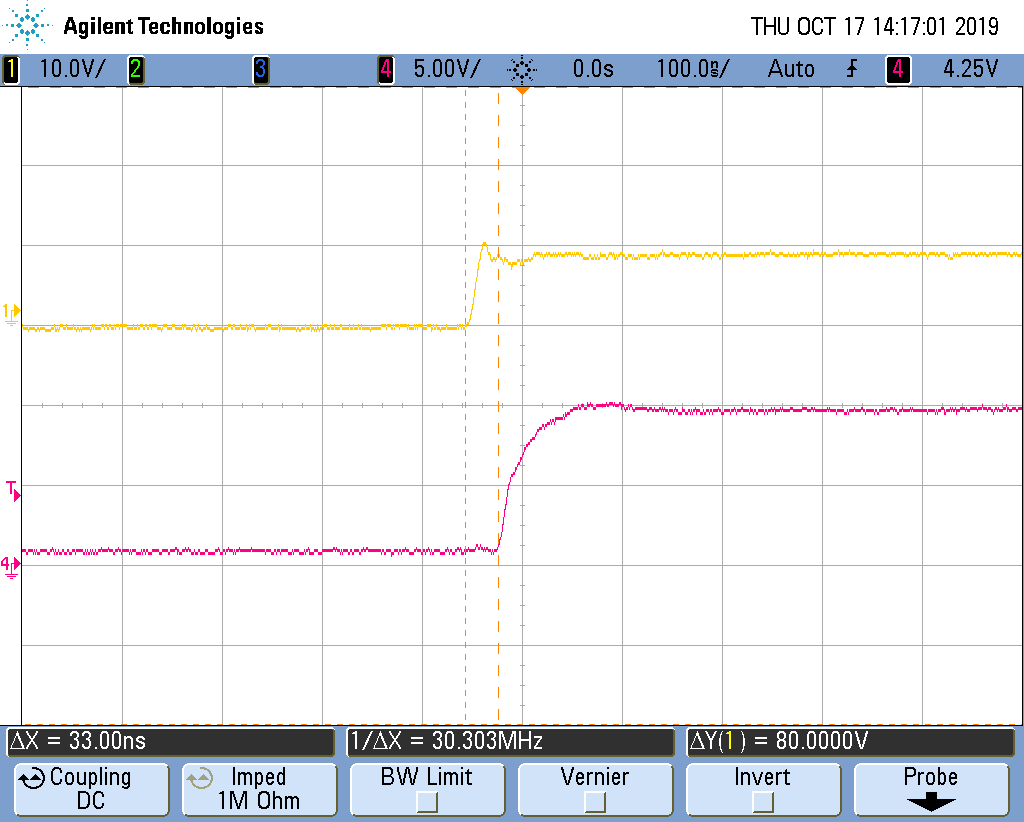
\includegraphics[width=0.8\textwidth]{Ejercicio7/Recursos/propagacion_sincronico.png}
	\caption{Propagacion contador sincr\'onico}
\end{figure}

En la siguiente captura se pueden ver las salidas de losdistintos fip-flops, el canal 1 corresponde al clock, y los canales 2, 3 y 4 corresponden a las salidas $Q_0$, $Q_1$ y $Q_2$ respectivamente:

\begin{figure}[H]
	\centering
	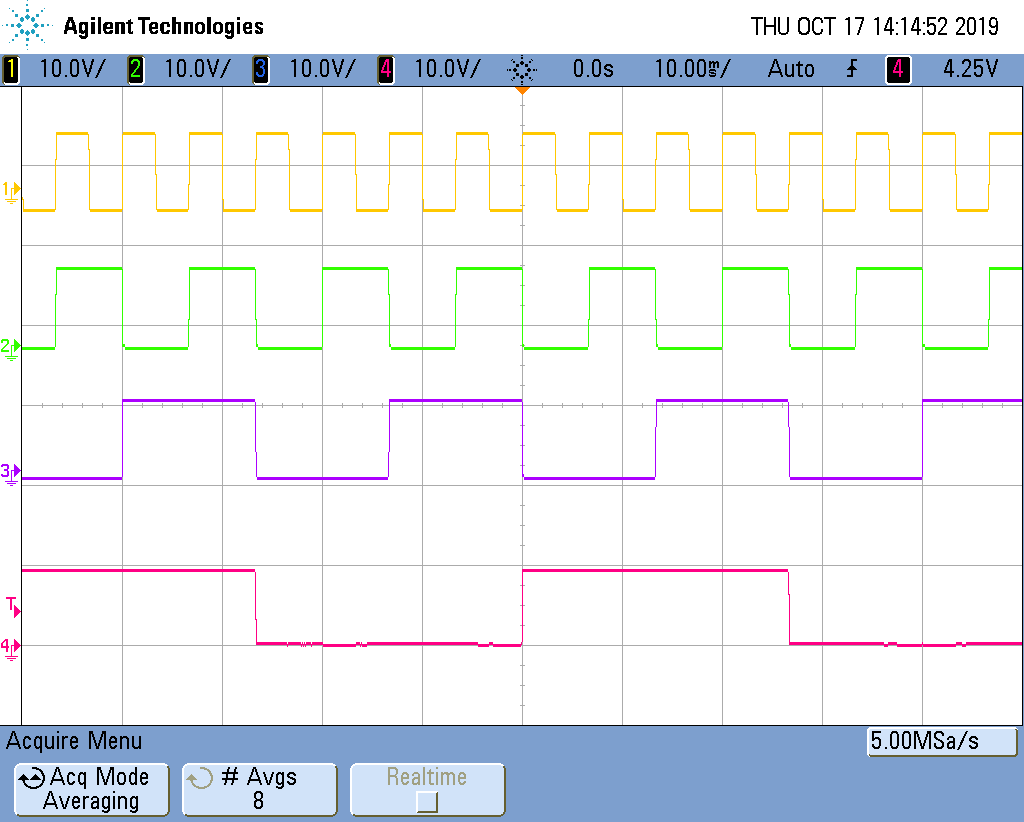
\includegraphics[width=0.8\textwidth]{Ejercicio7/Recursos/senales_sincronico.png}
	\caption{Diagrama de tiempo contador sincr\'onico}
\end{figure}

En el mismo se ve perfectamente como los flip-flops se prenden y apagan seg\'un la l\'ogica binaria del contador, del bit m\'as significatico al menos significativo.

En la siguiente tabla se resumen los resultados obtenidos para ambos contadores, importante denotar que para el contador asincr\'onico el tiempo de propagaci\'on que brinda el fabricante es de la salida $Q_n$ a $Q_{n+1}$:

\begin{table}[H]
\centering
\begin{tabular}{ll}\hline
\multicolumn{1}{c}{}           & Propagation Delay (ns) \\ \hline
Contador asicr\'onico comercial     &            $80-160$  \\
Contador asincr\'onico implementado        &       $220$  \\
Contador sincr\'onico comercial (MC14040) &         $25-75$ \\
Contador sincr\'onico implementado   &       $33$        \\  \hline
\end{tabular}
\end{table}

Salta a la vista que la hip'otesis inicial de que el contador asincr\'onico ser\'ia m\'as lento que el sincr\'onico se cumple, de hecho es 7 veces m\'as r\'apido. Adem\'as el valor para el tiempo de propagaci\'on del contador sincr\'onico queda dentro del rango bridnado por el fabricante.

 
\subsection{Conclusiones}
En el inicio del ejercicio se plantearon dos tipos de contadores ambos con ventajas y desventajas. Se plante\'o la hip\'otesis de que los sincr\'onicos ser\'ian mucho m\'as r\'apidos que los asincr\'onicos, debido a que en los \'ultimos no pueden ocurrir cambios en simult\'aneo ya que el clock debe propagarse por las distintas etapas. Se midieron ambos circuitos, y a pesar de que los resultaods emp\'iricos son distintos a los valores nominales de un circuito integrado en concreto, lo anterior puede deberse a eso mismo, los circuitos armados no est\'an integrados en el mismo chip de siicio y poseen propagaciones individuales mayores. Finalmente se confirm\'o la hip\'otesis incicial satisfactoriamente, por lo que, la velocidad de oepraci\'on de un contador esta dada por su tiepo de proagaci\'on y las misma es efectivamene menor para los contadores sincr\'onicos. 
